% TFF-Title: Weighted curved network
% TFF-Family: graph
% TFF-Tags: graph, weighted-network, curved-edges, edge-labels, textbook
% TFF-Description: Irregular weighted graph with readable curved edges and isolated edge labels.
% TFF-Origin: https://texample.net/tkz-berge/
% TFF-License: CC BY-SA 4.0
% TFF-Attribution: Adapted from Alain Matthes' tkz-berge example on TeXample.net
\documentclass[tikz,border=7pt]{standalone}
\usetikzlibrary{arrows.meta}
\begin{document}
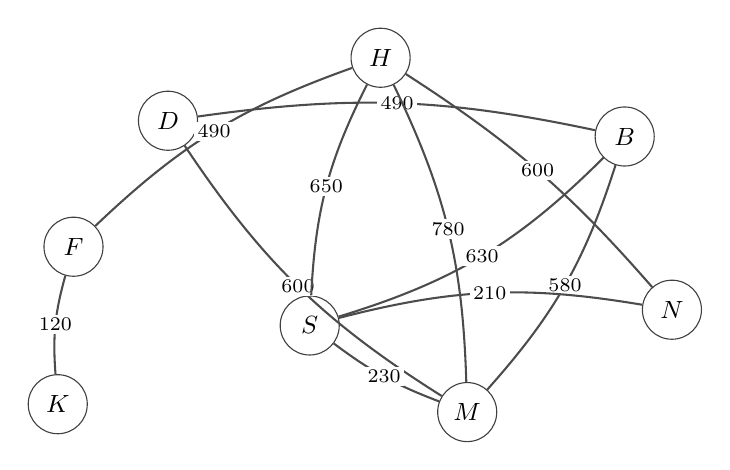
\begin{tikzpicture}[
  vertex/.style={circle,draw=black!75,fill=white,minimum size=7.5mm,inner sep=0pt,font=\small},
  edge/.style={draw=black!70,line width=.75pt},
  weight/.style={fill=white,inner sep=1.2pt,font=\scriptsize}
]
\node[vertex] (K) at (0,0) {$K$};
\node[vertex] (F) at (0.2,2.0) {$F$};
\node[vertex] (D) at (1.4,3.6) {$D$};
\node[vertex] (H) at (4.1,4.4) {$H$};
\node[vertex] (B) at (7.2,3.4) {$B$};
\node[vertex] (N) at (7.8,1.2) {$N$};
\node[vertex] (M) at (5.2,-0.1) {$M$};
\node[vertex] (S) at (3.2,1.0) {$S$};

\draw[edge] (K) to[bend left=10] node[weight] {120} (F);
\draw[edge] (F) to[bend left=12] node[weight] {490} (H);
\draw[edge] (D) to[bend left=10] node[weight] {490} (B);
\draw[edge] (D) to[bend right=12] node[weight] {600} (M);
\draw[edge] (H) to[bend left=12] node[weight] {780} (M);
\draw[edge] (H) to[bend left=8] node[weight] {600} (N);
\draw[edge] (H) to[bend right=12] node[weight] {650} (S);
\draw[edge] (B) to[bend left=12] node[weight] {580} (M);
\draw[edge] (S) to[bend right=14] node[weight] {630} (B);
\draw[edge] (S) to[bend left=12] node[weight] {210} (N);
\draw[edge] (S) to[bend right=8] node[weight] {230} (M);
\end{tikzpicture}
\end{document}
